\documentclass[twoside]{book}

% Packages required by doxygen
\usepackage{calc}
\usepackage{doxygen}
\usepackage{graphicx}
\usepackage[utf8]{inputenc}
\usepackage{makeidx}
\usepackage{multicol}
\usepackage{multirow}
\usepackage{textcomp}
\usepackage[table]{xcolor}

% NLS support packages
\usepackage[T2A]{fontenc}
\usepackage[czech]{babel}

% Font selection
\usepackage[T1]{fontenc}
\usepackage{mathptmx}
\usepackage[scaled=.90]{helvet}
\usepackage{courier}
\usepackage{amssymb}
\usepackage{sectsty}
\renewcommand{\familydefault}{\sfdefault}
\allsectionsfont{%
  \fontseries{bc}\selectfont%
  \color{darkgray}%
}
\renewcommand{\DoxyLabelFont}{%
  \fontseries{bc}\selectfont%
  \color{darkgray}%
}

% Page & text layout
\usepackage{geometry}
\geometry{%
  a4paper,%
  top=2.5cm,%
  bottom=2.5cm,%
  left=2.5cm,%
  right=2.5cm%
}
\tolerance=750
\hfuzz=15pt
\hbadness=750
\setlength{\emergencystretch}{15pt}
\setlength{\parindent}{0cm}
\setlength{\parskip}{0.2cm}
\makeatletter
\renewcommand{\paragraph}{%
  \@startsection{paragraph}{4}{0ex}{-1.0ex}{1.0ex}{%
    \normalfont\normalsize\bfseries\SS@parafont%
  }%
}
\renewcommand{\subparagraph}{%
  \@startsection{subparagraph}{5}{0ex}{-1.0ex}{1.0ex}{%
    \normalfont\normalsize\bfseries\SS@subparafont%
  }%
}
\makeatother

% Headers & footers
\usepackage{fancyhdr}
\pagestyle{fancyplain}
\fancyhead[LE]{\fancyplain{}{\bfseries\thepage}}
\fancyhead[CE]{\fancyplain{}{}}
\fancyhead[RE]{\fancyplain{}{\bfseries\leftmark}}
\fancyhead[LO]{\fancyplain{}{\bfseries\rightmark}}
\fancyhead[CO]{\fancyplain{}{}}
\fancyhead[RO]{\fancyplain{}{\bfseries\thepage}}
\fancyfoot[LE]{\fancyplain{}{}}
\fancyfoot[CE]{\fancyplain{}{}}
\fancyfoot[RE]{\fancyplain{}{\bfseries\scriptsize Generováno po 28. pro 2015 16.\-07\-:46 pro projekt Pastabin programem Doxygen }}
\fancyfoot[LO]{\fancyplain{}{\bfseries\scriptsize Generováno po 28. pro 2015 16.\-07\-:46 pro projekt Pastabin programem Doxygen }}
\fancyfoot[CO]{\fancyplain{}{}}
\fancyfoot[RO]{\fancyplain{}{}}
\renewcommand{\footrulewidth}{0.4pt}
\renewcommand{\chaptermark}[1]{%
  \markboth{#1}{}%
}
\renewcommand{\sectionmark}[1]{%
  \markright{\thesection\ #1}%
}

% Indices & bibliography
\usepackage{natbib}
\usepackage[titles]{tocloft}
\setcounter{tocdepth}{3}
\setcounter{secnumdepth}{5}
\makeindex

% Hyperlinks (required, but should be loaded last)
\usepackage{ifpdf}
\ifpdf
  \usepackage[pdftex,pagebackref=true]{hyperref}
\else
  \usepackage[ps2pdf,pagebackref=true]{hyperref}
\fi
\hypersetup{%
  colorlinks=true,%
  linkcolor=blue,%
  citecolor=blue,%
  unicode%
}

% Custom commands
\newcommand{\clearemptydoublepage}{%
  \newpage{\pagestyle{empty}\cleardoublepage}%
}


%===== C O N T E N T S =====

\begin{document}

% Titlepage & ToC
\hypersetup{pageanchor=false}
\pagenumbering{roman}
\begin{titlepage}
\vspace*{7cm}
\begin{center}%
{\Large Pastabin }\\
\vspace*{1cm}
{\large Generováno programem Doxygen 1.8.6}\\
\vspace*{0.5cm}
{\small po 28. pro 2015 16.07:46}\\
\end{center}
\end{titlepage}
\clearemptydoublepage
\tableofcontents
\clearemptydoublepage
\pagenumbering{arabic}
\hypersetup{pageanchor=true}

%--- Begin generated contents ---
\chapter{Rejstřík hierarchie tříd}
\section{Hierarchie tříd}
Zde naleznete seznam, vyjadřující vztah dědičnosti tříd. Je seřazen přibližně (ale ne úplně) podle abecedy\-:\begin{DoxyCompactList}
\item Exception\begin{DoxyCompactList}
\item \contentsline{section}{App\textbackslash{}Model\textbackslash{}Duplicate\-Name\-Exception}{\pageref{classApp_1_1Model_1_1DuplicateNameException}}{}
\end{DoxyCompactList}
\item I\-Authenticator\begin{DoxyCompactList}
\item \contentsline{section}{App\textbackslash{}Model\textbackslash{}User\-Manager}{\pageref{classApp_1_1Model_1_1UserManager}}{}
\end{DoxyCompactList}
\item I\-Presenter\begin{DoxyCompactList}
\item \contentsline{section}{App\textbackslash{}Presenters\textbackslash{}Error\-Presenter}{\pageref{classApp_1_1Presenters_1_1ErrorPresenter}}{}
\end{DoxyCompactList}
\item Object\begin{DoxyCompactList}
\item \contentsline{section}{App\textbackslash{}Forms\textbackslash{}Sign\-Form\-Factory}{\pageref{classApp_1_1Forms_1_1SignFormFactory}}{}
\item \contentsline{section}{App\textbackslash{}Model\textbackslash{}Base}{\pageref{classApp_1_1Model_1_1Base}}{}
\begin{DoxyCompactList}
\item \contentsline{section}{App\textbackslash{}Model\textbackslash{}Pasters}{\pageref{classApp_1_1Model_1_1Pasters}}{}
\end{DoxyCompactList}
\item \contentsline{section}{App\textbackslash{}Model\textbackslash{}User\-Manager}{\pageref{classApp_1_1Model_1_1UserManager}}{}
\item \contentsline{section}{App\textbackslash{}Presenters\textbackslash{}Error\-Presenter}{\pageref{classApp_1_1Presenters_1_1ErrorPresenter}}{}
\end{DoxyCompactList}
\item Presenter\begin{DoxyCompactList}
\item \contentsline{section}{App\textbackslash{}Presenters\textbackslash{}Base\-Presenter}{\pageref{classApp_1_1Presenters_1_1BasePresenter}}{}
\begin{DoxyCompactList}
\item \contentsline{section}{App\textbackslash{}Presenters\textbackslash{}Error4xx\-Presenter}{\pageref{classApp_1_1Presenters_1_1Error4xxPresenter}}{}
\item \contentsline{section}{App\textbackslash{}Presenters\textbackslash{}Homepage\-Presenter}{\pageref{classApp_1_1Presenters_1_1HomepagePresenter}}{}
\item \contentsline{section}{App\textbackslash{}Presenters\textbackslash{}Pastes\-Presenter}{\pageref{classApp_1_1Presenters_1_1PastesPresenter}}{}
\item \contentsline{section}{App\textbackslash{}Presenters\textbackslash{}Sign\-Presenter}{\pageref{classApp_1_1Presenters_1_1SignPresenter}}{}
\end{DoxyCompactList}
\end{DoxyCompactList}
\item \contentsline{section}{App\textbackslash{}Router\-Factory}{\pageref{classApp_1_1RouterFactory}}{}
\end{DoxyCompactList}

\chapter{Rejstřík tříd}
\section{Seznam tříd}
Následující seznam obsahuje především identifikace tříd, ale nacházejí se zde i další netriviální prvky, jako jsou struktury (struct), unie (union) a rozhraní (interface). V seznamu jsou uvedeny jejich stručné popisy\-:\begin{DoxyCompactList}
\item\contentsline{section}{\hyperlink{classApp_1_1Model_1_1Base}{App\textbackslash{}\-Model\textbackslash{}\-Base} \\*Hlavní model volající databázi }{\pageref{classApp_1_1Model_1_1Base}}{}
\item\contentsline{section}{\hyperlink{classApp_1_1Presenters_1_1BasePresenter}{App\textbackslash{}\-Presenters\textbackslash{}\-Base\-Presenter} \\*Hlavní prezentér }{\pageref{classApp_1_1Presenters_1_1BasePresenter}}{}
\item\contentsline{section}{\hyperlink{classApp_1_1Model_1_1DuplicateNameException}{App\textbackslash{}\-Model\textbackslash{}\-Duplicate\-Name\-Exception} }{\pageref{classApp_1_1Model_1_1DuplicateNameException}}{}
\item\contentsline{section}{\hyperlink{classApp_1_1Presenters_1_1Error4xxPresenter}{App\textbackslash{}\-Presenters\textbackslash{}\-Error4xx\-Presenter} }{\pageref{classApp_1_1Presenters_1_1Error4xxPresenter}}{}
\item\contentsline{section}{\hyperlink{classApp_1_1Presenters_1_1ErrorPresenter}{App\textbackslash{}\-Presenters\textbackslash{}\-Error\-Presenter} }{\pageref{classApp_1_1Presenters_1_1ErrorPresenter}}{}
\item\contentsline{section}{\hyperlink{classApp_1_1Presenters_1_1HomepagePresenter}{App\textbackslash{}\-Presenters\textbackslash{}\-Homepage\-Presenter} \\*Prezentér pracující s hlavní stránkou }{\pageref{classApp_1_1Presenters_1_1HomepagePresenter}}{}
\item\contentsline{section}{\hyperlink{classApp_1_1Model_1_1Pasters}{App\textbackslash{}\-Model\textbackslash{}\-Pasters} \\*Model reprezentující entitu pastes z databáze }{\pageref{classApp_1_1Model_1_1Pasters}}{}
\item\contentsline{section}{\hyperlink{classApp_1_1Presenters_1_1PastesPresenter}{App\textbackslash{}\-Presenters\textbackslash{}\-Pastes\-Presenter} \\*Prezentér pro pasty }{\pageref{classApp_1_1Presenters_1_1PastesPresenter}}{}
\item\contentsline{section}{\hyperlink{classApp_1_1RouterFactory}{App\textbackslash{}\-Router\-Factory} }{\pageref{classApp_1_1RouterFactory}}{}
\item\contentsline{section}{\hyperlink{classApp_1_1Forms_1_1SignFormFactory}{App\textbackslash{}\-Forms\textbackslash{}\-Sign\-Form\-Factory} }{\pageref{classApp_1_1Forms_1_1SignFormFactory}}{}
\item\contentsline{section}{\hyperlink{classApp_1_1Presenters_1_1SignPresenter}{App\textbackslash{}\-Presenters\textbackslash{}\-Sign\-Presenter} }{\pageref{classApp_1_1Presenters_1_1SignPresenter}}{}
\item\contentsline{section}{\hyperlink{classApp_1_1Model_1_1UserManager}{App\textbackslash{}\-Model\textbackslash{}\-User\-Manager} }{\pageref{classApp_1_1Model_1_1UserManager}}{}
\end{DoxyCompactList}

\chapter{Dokumentace tříd}
\hypertarget{classApp_1_1Model_1_1Base}{\section{Dokumentace třídy App\textbackslash{}Model\textbackslash{}Base}
\label{classApp_1_1Model_1_1Base}\index{App\textbackslash{}\-Model\textbackslash{}\-Base@{App\textbackslash{}\-Model\textbackslash{}\-Base}}
}


Hlavní model volající databázi.  


Diagram dědičnosti pro třídu App\textbackslash{}Model\textbackslash{}Base\begin{figure}[H]
\begin{center}
\leavevmode
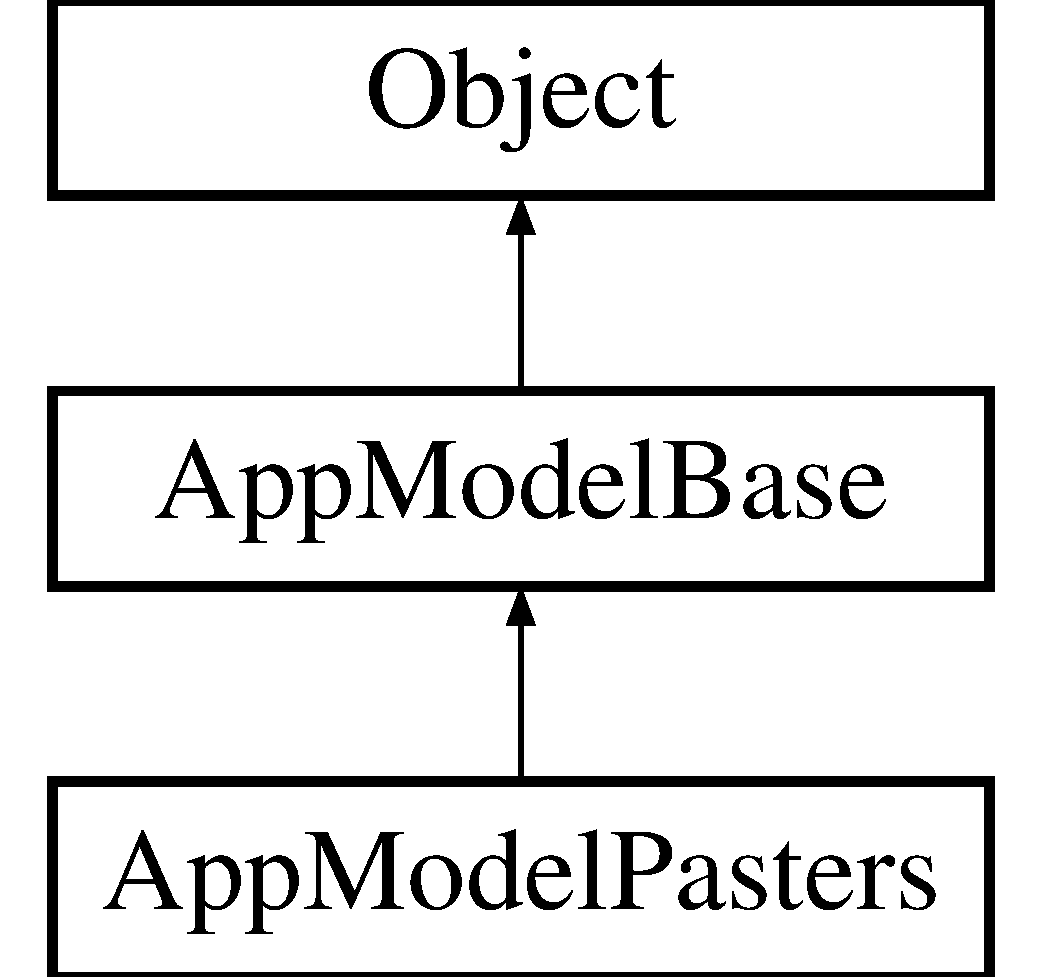
\includegraphics[height=3.000000cm]{classApp_1_1Model_1_1Base}
\end{center}
\end{figure}
\subsection*{Veřejné metody}
\begin{DoxyCompactItemize}
\item 
\hypertarget{classApp_1_1Model_1_1Base_a9cdb951ad2ab48fb8661f8db19527596}{{\bfseries \-\_\-\-\_\-construct} (Nette\textbackslash{}\-Database\textbackslash{}\-Context \$database)}\label{classApp_1_1Model_1_1Base_a9cdb951ad2ab48fb8661f8db19527596}

\end{DoxyCompactItemize}
\subsection*{Chráněné atributy}
\begin{DoxyCompactItemize}
\item 
\hypertarget{classApp_1_1Model_1_1Base_af3c545dcc02fdfc450ec0a20a24148d5}{{\bfseries \$database}}\label{classApp_1_1Model_1_1Base_af3c545dcc02fdfc450ec0a20a24148d5}

\end{DoxyCompactItemize}


\subsection{Detailní popis}
Hlavní model volající databázi. 

Dokumentace pro tuto třídu byla generována z následujícího souboru\-:\begin{DoxyCompactItemize}
\item 
model/Base\-Model.\-php\end{DoxyCompactItemize}

\hypertarget{classApp_1_1Presenters_1_1BasePresenter}{\section{Dokumentace třídy App\textbackslash{}Presenters\textbackslash{}Base\-Presenter}
\label{classApp_1_1Presenters_1_1BasePresenter}\index{App\textbackslash{}\-Presenters\textbackslash{}\-Base\-Presenter@{App\textbackslash{}\-Presenters\textbackslash{}\-Base\-Presenter}}
}


Hlavní prezentér.  


Diagram dědičnosti pro třídu App\textbackslash{}Presenters\textbackslash{}Base\-Presenter\begin{figure}[H]
\begin{center}
\leavevmode
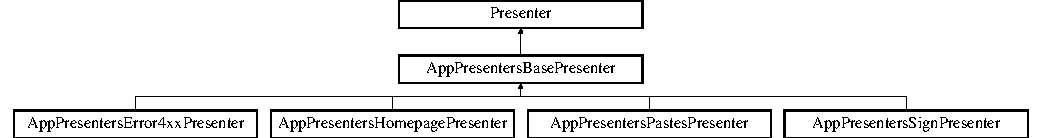
\includegraphics[height=1.850220cm]{classApp_1_1Presenters_1_1BasePresenter}
\end{center}
\end{figure}


\subsection{Detailní popis}
Hlavní prezentér. 

Dokumentace pro tuto třídu byla generována z následujícího souboru\-:\begin{DoxyCompactItemize}
\item 
presenters/Base\-Presenter.\-php\end{DoxyCompactItemize}

\hypertarget{classApp_1_1Model_1_1DuplicateNameException}{\section{Dokumentace třídy App\textbackslash{}Model\textbackslash{}Duplicate\-Name\-Exception}
\label{classApp_1_1Model_1_1DuplicateNameException}\index{App\textbackslash{}\-Model\textbackslash{}\-Duplicate\-Name\-Exception@{App\textbackslash{}\-Model\textbackslash{}\-Duplicate\-Name\-Exception}}
}
Diagram dědičnosti pro třídu App\textbackslash{}Model\textbackslash{}Duplicate\-Name\-Exception\begin{figure}[H]
\begin{center}
\leavevmode
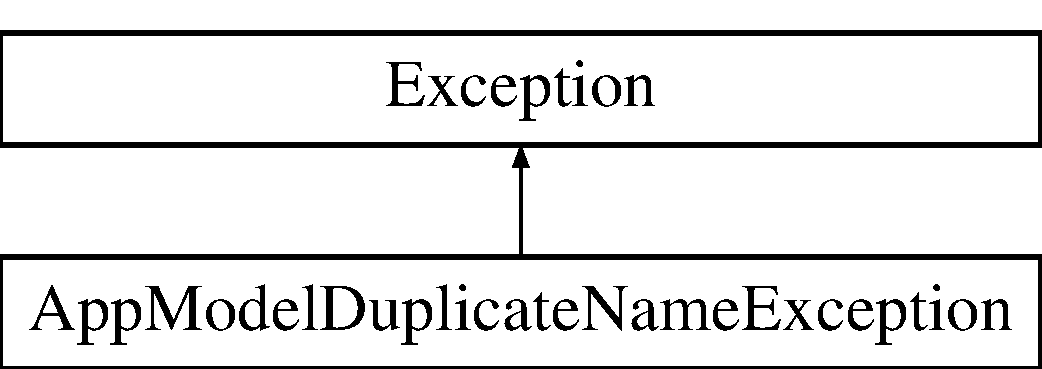
\includegraphics[height=2.000000cm]{classApp_1_1Model_1_1DuplicateNameException}
\end{center}
\end{figure}


Dokumentace pro tuto třídu byla generována z následujícího souboru\-:\begin{DoxyCompactItemize}
\item 
model/User\-Manager.\-php\end{DoxyCompactItemize}

\hypertarget{classApp_1_1Presenters_1_1Error4xxPresenter}{\section{Dokumentace třídy App\textbackslash{}Presenters\textbackslash{}Error4xx\-Presenter}
\label{classApp_1_1Presenters_1_1Error4xxPresenter}\index{App\textbackslash{}\-Presenters\textbackslash{}\-Error4xx\-Presenter@{App\textbackslash{}\-Presenters\textbackslash{}\-Error4xx\-Presenter}}
}
Diagram dědičnosti pro třídu App\textbackslash{}Presenters\textbackslash{}Error4xx\-Presenter\begin{figure}[H]
\begin{center}
\leavevmode
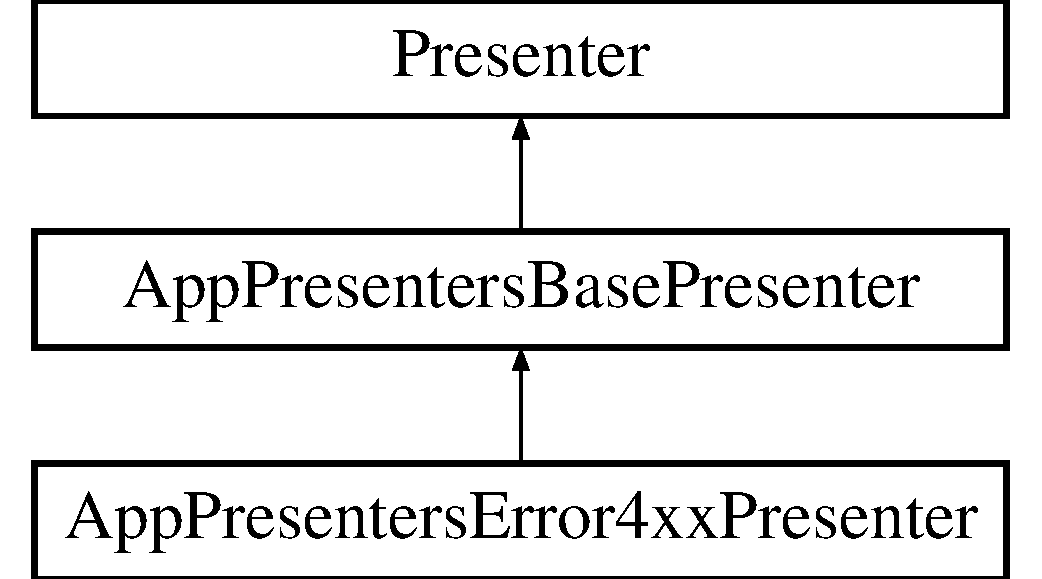
\includegraphics[height=3.000000cm]{classApp_1_1Presenters_1_1Error4xxPresenter}
\end{center}
\end{figure}
\subsection*{Veřejné metody}
\begin{DoxyCompactItemize}
\item 
\hypertarget{classApp_1_1Presenters_1_1Error4xxPresenter_a74554da47cce26e25d783141c95da87b}{{\bfseries startup} ()}\label{classApp_1_1Presenters_1_1Error4xxPresenter_a74554da47cce26e25d783141c95da87b}

\item 
\hypertarget{classApp_1_1Presenters_1_1Error4xxPresenter_a7b1526f98943508230687ae594873c1d}{{\bfseries render\-Default} (Nette\textbackslash{}\-Application\textbackslash{}\-Bad\-Request\-Exception \$exception)}\label{classApp_1_1Presenters_1_1Error4xxPresenter_a7b1526f98943508230687ae594873c1d}

\end{DoxyCompactItemize}


Dokumentace pro tuto třídu byla generována z následujícího souboru\-:\begin{DoxyCompactItemize}
\item 
presenters/Error4xx\-Presenter.\-php\end{DoxyCompactItemize}

\hypertarget{classApp_1_1Presenters_1_1ErrorPresenter}{\section{Dokumentace třídy App\textbackslash{}Presenters\textbackslash{}Error\-Presenter}
\label{classApp_1_1Presenters_1_1ErrorPresenter}\index{App\textbackslash{}\-Presenters\textbackslash{}\-Error\-Presenter@{App\textbackslash{}\-Presenters\textbackslash{}\-Error\-Presenter}}
}
Diagram dědičnosti pro třídu App\textbackslash{}Presenters\textbackslash{}Error\-Presenter\begin{figure}[H]
\begin{center}
\leavevmode
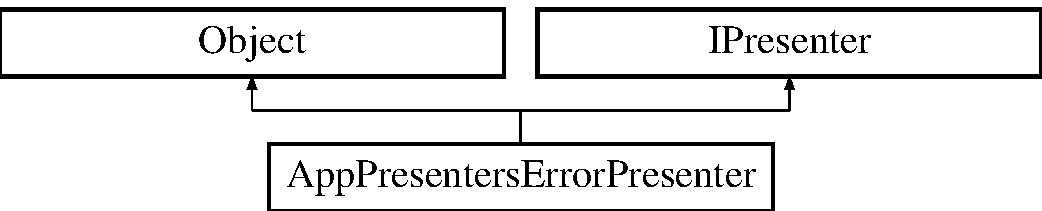
\includegraphics[height=2.000000cm]{classApp_1_1Presenters_1_1ErrorPresenter}
\end{center}
\end{figure}
\subsection*{Veřejné metody}
\begin{DoxyCompactItemize}
\item 
\hypertarget{classApp_1_1Presenters_1_1ErrorPresenter_a654d7865f7d6c2d8386e63f1139f3274}{{\bfseries \-\_\-\-\_\-construct} (I\-Logger \$logger)}\label{classApp_1_1Presenters_1_1ErrorPresenter_a654d7865f7d6c2d8386e63f1139f3274}

\item 
\hyperlink{classApp_1_1Presenters_1_1ErrorPresenter_adc5204ef5298be3322789e1ddbc443fb}{run} (Nette\textbackslash{}\-Application\textbackslash{}\-Request \$request)
\end{DoxyCompactItemize}


\subsection{Dokumentace k metodám}
\hypertarget{classApp_1_1Presenters_1_1ErrorPresenter_adc5204ef5298be3322789e1ddbc443fb}{\index{App\-::\-Presenters\-::\-Error\-Presenter@{App\-::\-Presenters\-::\-Error\-Presenter}!run@{run}}
\index{run@{run}!App::Presenters::ErrorPresenter@{App\-::\-Presenters\-::\-Error\-Presenter}}
\subsubsection[{run}]{\setlength{\rightskip}{0pt plus 5cm}App\textbackslash{}\-Presenters\textbackslash{}\-Error\-Presenter\-::run (
\begin{DoxyParamCaption}
\item[{Nette\textbackslash{}\-Application\textbackslash{}\-Request}]{\$request}
\end{DoxyParamCaption}
)}}\label{classApp_1_1Presenters_1_1ErrorPresenter_adc5204ef5298be3322789e1ddbc443fb}
\begin{DoxyReturn}{Návratová hodnota}
Nette 
\end{DoxyReturn}


Dokumentace pro tuto třídu byla generována z následujícího souboru\-:\begin{DoxyCompactItemize}
\item 
app/presenters/Error\-Presenter.\-php\end{DoxyCompactItemize}

\hypertarget{classApp_1_1Presenters_1_1HomepagePresenter}{\section{Dokumentace třídy App\textbackslash{}Presenters\textbackslash{}Homepage\-Presenter}
\label{classApp_1_1Presenters_1_1HomepagePresenter}\index{App\textbackslash{}\-Presenters\textbackslash{}\-Homepage\-Presenter@{App\textbackslash{}\-Presenters\textbackslash{}\-Homepage\-Presenter}}
}


Prezentér pracující s hlavní stránkou.  


Diagram dědičnosti pro třídu App\textbackslash{}Presenters\textbackslash{}Homepage\-Presenter\begin{figure}[H]
\begin{center}
\leavevmode
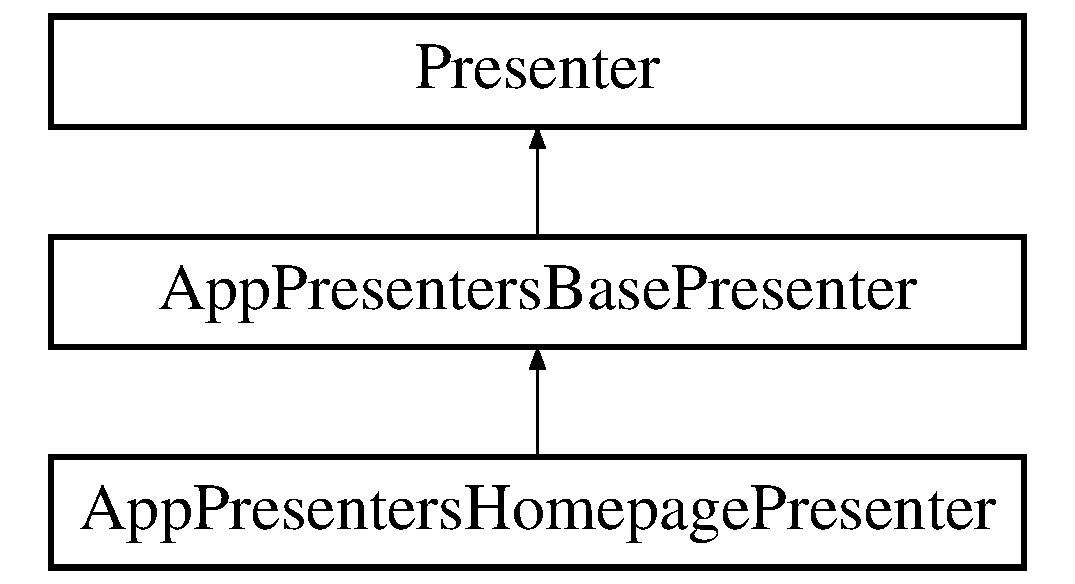
\includegraphics[height=3.000000cm]{classApp_1_1Presenters_1_1HomepagePresenter}
\end{center}
\end{figure}
\subsection*{Veřejné metody}
\begin{DoxyCompactItemize}
\item 
\hyperlink{classApp_1_1Presenters_1_1HomepagePresenter_a9f3ca2d8ad95a60ccbcce5566eb2a1f3}{inject\-Models} (\hyperlink{classApp_1_1Model_1_1Pasters}{Model\textbackslash{}\-Pasters} \$\hyperlink{classApp_1_1Model_1_1Pasters}{Pasters}, \hyperlink{classApp_1_1Model_1_1UserManager}{Model\textbackslash{}\-User\-Manager} \$user\-Manager)
\begin{DoxyCompactList}\small\item\em Metoda vytvoří pomocí injekce model mapující databázi. \end{DoxyCompactList}\item 
\hypertarget{classApp_1_1Presenters_1_1HomepagePresenter_a6903224ecfc8b81b2ab3269f574da84f}{\hyperlink{classApp_1_1Presenters_1_1HomepagePresenter_a6903224ecfc8b81b2ab3269f574da84f}{render\-Default} ()}\label{classApp_1_1Presenters_1_1HomepagePresenter_a6903224ecfc8b81b2ab3269f574da84f}

\begin{DoxyCompactList}\small\item\em Metoda pro konstrukci proměnných určených pro pohledy. \end{DoxyCompactList}\item 
\hyperlink{classApp_1_1Presenters_1_1HomepagePresenter_af63c0f54a5c4f89f36efecc4a84b8366}{login\-Form\-Succeeded} (U\-I\textbackslash{}\-Form \$form, \$values)
\begin{DoxyCompactList}\small\item\em Metoda vyhodnotí výsledky odeslaného formuláře. \end{DoxyCompactList}\item 
\hypertarget{classApp_1_1Presenters_1_1HomepagePresenter_aeb9f0e1d86324ec6d824b4b3de07cec7}{{\bfseries Action\-Logout} ()}\label{classApp_1_1Presenters_1_1HomepagePresenter_aeb9f0e1d86324ec6d824b4b3de07cec7}

\item 
\hypertarget{classApp_1_1Presenters_1_1HomepagePresenter_a8b8ecf6b3adccfc0d094586c48c27194}{{\bfseries Action\-Removeme} ()}\label{classApp_1_1Presenters_1_1HomepagePresenter_a8b8ecf6b3adccfc0d094586c48c27194}

\item 
\hypertarget{classApp_1_1Presenters_1_1HomepagePresenter_a21a1f43ddd9f04bf126fbb59670c64ad}{{\bfseries paste\-Form\-Succeeded} (U\-I\textbackslash{}\-Form \$form, \$values)}\label{classApp_1_1Presenters_1_1HomepagePresenter_a21a1f43ddd9f04bf126fbb59670c64ad}

\end{DoxyCompactItemize}
\subsection*{Chráněné metody}
\begin{DoxyCompactItemize}
\item 
\hypertarget{classApp_1_1Presenters_1_1HomepagePresenter_afd1a8f72e16c8ded158b074e049c2a1c}{\hyperlink{classApp_1_1Presenters_1_1HomepagePresenter_afd1a8f72e16c8ded158b074e049c2a1c}{create\-Component\-Paste\-Form} ()}\label{classApp_1_1Presenters_1_1HomepagePresenter_afd1a8f72e16c8ded158b074e049c2a1c}

\begin{DoxyCompactList}\small\item\em Metoda pro konstrukci komponenty formuláře. Nastaví relaci na Java\-Script funkci adjust. \end{DoxyCompactList}\item 
\hypertarget{classApp_1_1Presenters_1_1HomepagePresenter_aee7e1fb56dcb24a048c803796706d89a}{\hyperlink{classApp_1_1Presenters_1_1HomepagePresenter_aee7e1fb56dcb24a048c803796706d89a}{create\-Component\-Login\-Form} ()}\label{classApp_1_1Presenters_1_1HomepagePresenter_aee7e1fb56dcb24a048c803796706d89a}

\begin{DoxyCompactList}\small\item\em Metoda volaná po odeslání formuláře. \end{DoxyCompactList}\end{DoxyCompactItemize}


\subsection{Detailní popis}
Prezentér pracující s hlavní stránkou. 

\subsection{Dokumentace k metodám}
\hypertarget{classApp_1_1Presenters_1_1HomepagePresenter_a9f3ca2d8ad95a60ccbcce5566eb2a1f3}{\index{App\-::\-Presenters\-::\-Homepage\-Presenter@{App\-::\-Presenters\-::\-Homepage\-Presenter}!inject\-Models@{inject\-Models}}
\index{inject\-Models@{inject\-Models}!App::Presenters::HomepagePresenter@{App\-::\-Presenters\-::\-Homepage\-Presenter}}
\subsubsection[{inject\-Models}]{\setlength{\rightskip}{0pt plus 5cm}App\textbackslash{}\-Presenters\textbackslash{}\-Homepage\-Presenter\-::inject\-Models (
\begin{DoxyParamCaption}
\item[{{\bf Model\textbackslash{}\-Pasters}}]{\$\-Pasters, }
\item[{{\bf Model\textbackslash{}\-User\-Manager}}]{\$user\-Manager}
\end{DoxyParamCaption}
)}}\label{classApp_1_1Presenters_1_1HomepagePresenter_a9f3ca2d8ad95a60ccbcce5566eb2a1f3}


Metoda vytvoří pomocí injekce model mapující databázi. 


\begin{DoxyParams}[1]{Parametry}
\mbox{\tt in}  & {\em \$\-Pasters} & injekce modelu \\
\hline
\mbox{\tt in}  & {\em \$user\-Manager} & injekce modelu \\
\hline
\end{DoxyParams}
\hypertarget{classApp_1_1Presenters_1_1HomepagePresenter_af63c0f54a5c4f89f36efecc4a84b8366}{\index{App\-::\-Presenters\-::\-Homepage\-Presenter@{App\-::\-Presenters\-::\-Homepage\-Presenter}!login\-Form\-Succeeded@{login\-Form\-Succeeded}}
\index{login\-Form\-Succeeded@{login\-Form\-Succeeded}!App::Presenters::HomepagePresenter@{App\-::\-Presenters\-::\-Homepage\-Presenter}}
\subsubsection[{login\-Form\-Succeeded}]{\setlength{\rightskip}{0pt plus 5cm}App\textbackslash{}\-Presenters\textbackslash{}\-Homepage\-Presenter\-::login\-Form\-Succeeded (
\begin{DoxyParamCaption}
\item[{U\-I\textbackslash{}\-Form}]{\$form, }
\item[{}]{\$values}
\end{DoxyParamCaption}
)}}\label{classApp_1_1Presenters_1_1HomepagePresenter_af63c0f54a5c4f89f36efecc4a84b8366}


Metoda vyhodnotí výsledky odeslaného formuláře. 

Metoda vloží paste do databáze a odešle uživatele na další prezentér.


\begin{DoxyParams}[1]{Parametry}
\mbox{\tt in}  & {\em \$form} & objekt formuláře \\
\hline
\mbox{\tt in}  & {\em \$values} & data z formuláře \\
\hline
\end{DoxyParams}


Dokumentace pro tuto třídu byla generována z následujícího souboru\-:\begin{DoxyCompactItemize}
\item 
app/presenters/Homepage\-Presenter.\-php\end{DoxyCompactItemize}

\hypertarget{classApp_1_1Model_1_1Pasters}{\section{Dokumentace třídy App\textbackslash{}Model\textbackslash{}Pasters}
\label{classApp_1_1Model_1_1Pasters}\index{App\textbackslash{}\-Model\textbackslash{}\-Pasters@{App\textbackslash{}\-Model\textbackslash{}\-Pasters}}
}


Model reprezentující entitu pastes z databáze.  


Diagram dědičnosti pro třídu App\textbackslash{}Model\textbackslash{}Pasters\begin{figure}[H]
\begin{center}
\leavevmode
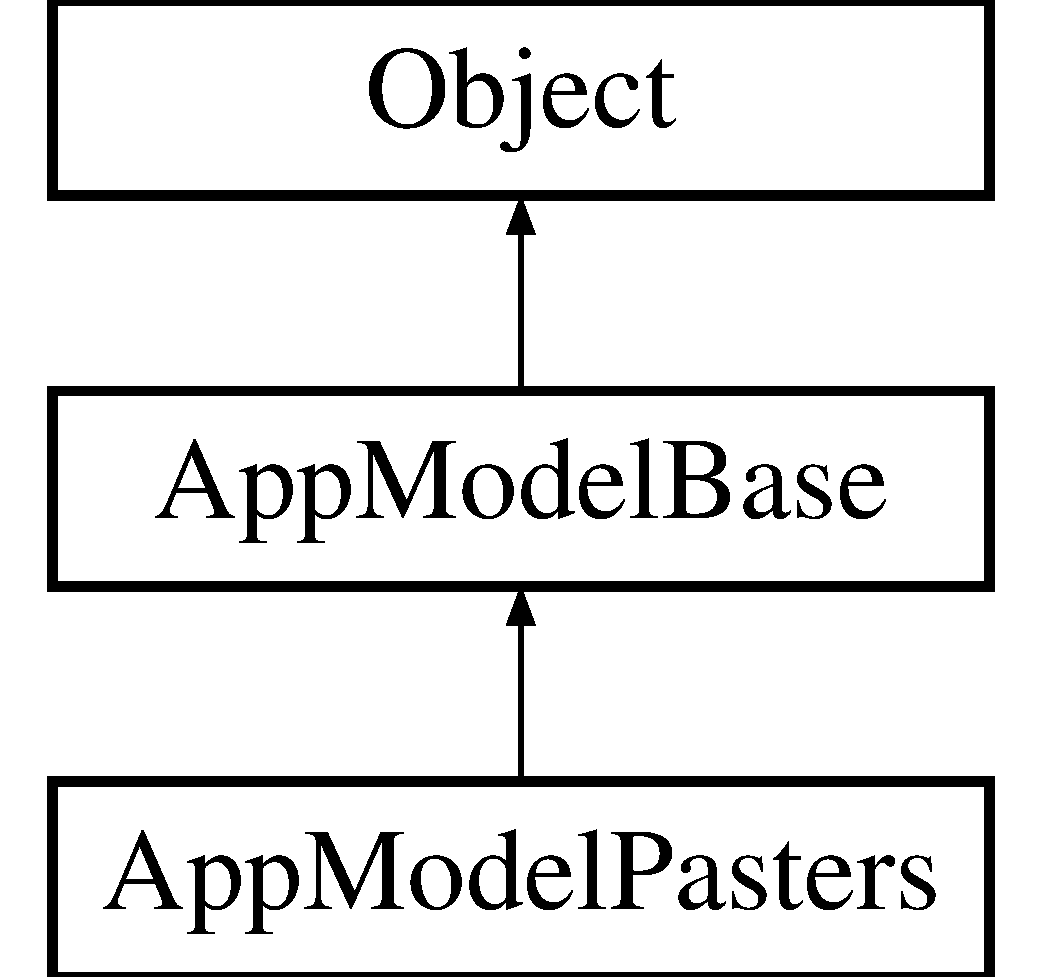
\includegraphics[height=3.000000cm]{classApp_1_1Model_1_1Pasters}
\end{center}
\end{figure}
\subsection*{Veřejné metody}
\begin{DoxyCompactItemize}
\item 
\hyperlink{classApp_1_1Model_1_1Pasters_a778c4b70c0f01cfbc8e5dc501cc2690a}{add} (\$value, \$id\-\_\-user)
\begin{DoxyCompactList}\small\item\em Metoda vytvoří paste v databázi a vyhodí excepšnu při chybě \end{DoxyCompactList}\item 
\hyperlink{classApp_1_1Model_1_1Pasters_aa16e80c8cde9bb0fb3297b7d0d9ec811}{find\-By} (array \$by)
\begin{DoxyCompactList}\small\item\em Metoda prohledá tabulku podle kritérií v \$by. \end{DoxyCompactList}\item 
\hyperlink{classApp_1_1Model_1_1Pasters_a541268fec1aa42f6e01f27c9cf898d68}{update} (\$data)
\begin{DoxyCompactList}\small\item\em Metoda změní data podle vstupního id. \end{DoxyCompactList}\item 
\hyperlink{classApp_1_1Model_1_1Pasters_aa411c7eb5396b9a3b3a94fd0b906d7d5}{del} (\$id)
\begin{DoxyCompactList}\small\item\em Metoda smaže záznam podle \$id. \end{DoxyCompactList}\item 
\hyperlink{classApp_1_1Model_1_1Pasters_a4490387bc6ed706b7fbac89a90d34786}{del\-By\-User} (\$userid)
\begin{DoxyCompactList}\small\item\em Metoda smaže vše, co patřilo uživateli podle id. \end{DoxyCompactList}\item 
\hyperlink{classApp_1_1Model_1_1Pasters_ae229992c1cb37e23b8ba08559cdae953}{get\-Table} ()
\begin{DoxyCompactList}\small\item\em Metoda vrátí celou tabulku. \end{DoxyCompactList}\item 
\hyperlink{classApp_1_1Model_1_1Pasters_a8e8331fb00d3369398bcbbe06822ee7c}{get\-Line} (\$id)
\begin{DoxyCompactList}\small\item\em Metoda vrátí řádek podle id. \end{DoxyCompactList}\item 
\hyperlink{classApp_1_1Model_1_1Pasters_ad7c8c8fae5bd7d13799bc0d08a4896eb}{get\-By\-User} (\$id)
\begin{DoxyCompactList}\small\item\em Metoda vrátí vše podle id uživatele. \end{DoxyCompactList}\item 
\hyperlink{classApp_1_1Model_1_1Pasters_a6c7ab1c9e478f59efdb380401666dabc}{get\-Line\-By\-User\-Id} (\$id)
\begin{DoxyCompactList}\small\item\em Metoda vrátí vše podle id uživatele. \end{DoxyCompactList}\end{DoxyCompactItemize}
\subsection*{Veřejné atributy}
\begin{DoxyCompactItemize}
\item 
\hypertarget{classApp_1_1Model_1_1Pasters_a437b6b51a7609885ccf5a13e6ab6ea7a}{const \hyperlink{classApp_1_1Model_1_1Pasters_a437b6b51a7609885ccf5a13e6ab6ea7a}{T\-A\-B\-L\-E\-\_\-\-N\-A\-M\-E} = 'pastes'}\label{classApp_1_1Model_1_1Pasters_a437b6b51a7609885ccf5a13e6ab6ea7a}

\begin{DoxyCompactList}\small\item\em Jméno tabulky. \end{DoxyCompactList}\end{DoxyCompactItemize}
\subsection*{Další zděděné členy}


\subsection{Detailní popis}
Model reprezentující entitu pastes z databáze. 

\subsection{Dokumentace k metodám}
\hypertarget{classApp_1_1Model_1_1Pasters_a778c4b70c0f01cfbc8e5dc501cc2690a}{\index{App\-::\-Model\-::\-Pasters@{App\-::\-Model\-::\-Pasters}!add@{add}}
\index{add@{add}!App::Model::Pasters@{App\-::\-Model\-::\-Pasters}}
\subsubsection[{add}]{\setlength{\rightskip}{0pt plus 5cm}App\textbackslash{}\-Model\textbackslash{}\-Pasters\-::add (
\begin{DoxyParamCaption}
\item[{}]{\$value, }
\item[{}]{\$id\-\_\-user}
\end{DoxyParamCaption}
)}}\label{classApp_1_1Model_1_1Pasters_a778c4b70c0f01cfbc8e5dc501cc2690a}


Metoda vytvoří paste v databázi a vyhodí excepšnu při chybě 


\begin{DoxyParams}[1]{Parametry}
\mbox{\tt in}  & {\em \$value} & data pastu \\
\hline
\mbox{\tt in}  & {\em \$id\-\_\-user} & id uživatele \\
\hline
\end{DoxyParams}
\hypertarget{classApp_1_1Model_1_1Pasters_aa411c7eb5396b9a3b3a94fd0b906d7d5}{\index{App\-::\-Model\-::\-Pasters@{App\-::\-Model\-::\-Pasters}!del@{del}}
\index{del@{del}!App::Model::Pasters@{App\-::\-Model\-::\-Pasters}}
\subsubsection[{del}]{\setlength{\rightskip}{0pt plus 5cm}App\textbackslash{}\-Model\textbackslash{}\-Pasters\-::del (
\begin{DoxyParamCaption}
\item[{}]{\$id}
\end{DoxyParamCaption}
)}}\label{classApp_1_1Model_1_1Pasters_aa411c7eb5396b9a3b3a94fd0b906d7d5}


Metoda smaže záznam podle \$id. 


\begin{DoxyParams}[1]{Parametry}
\mbox{\tt in}  & {\em \$id} & záznamu ke smazání \\
\hline
\end{DoxyParams}
\hypertarget{classApp_1_1Model_1_1Pasters_a4490387bc6ed706b7fbac89a90d34786}{\index{App\-::\-Model\-::\-Pasters@{App\-::\-Model\-::\-Pasters}!del\-By\-User@{del\-By\-User}}
\index{del\-By\-User@{del\-By\-User}!App::Model::Pasters@{App\-::\-Model\-::\-Pasters}}
\subsubsection[{del\-By\-User}]{\setlength{\rightskip}{0pt plus 5cm}App\textbackslash{}\-Model\textbackslash{}\-Pasters\-::del\-By\-User (
\begin{DoxyParamCaption}
\item[{}]{\$userid}
\end{DoxyParamCaption}
)}}\label{classApp_1_1Model_1_1Pasters_a4490387bc6ed706b7fbac89a90d34786}


Metoda smaže vše, co patřilo uživateli podle id. 


\begin{DoxyParams}[1]{Parametry}
\mbox{\tt in}  & {\em \$userid} & id uživatele \\
\hline
\end{DoxyParams}
\hypertarget{classApp_1_1Model_1_1Pasters_aa16e80c8cde9bb0fb3297b7d0d9ec811}{\index{App\-::\-Model\-::\-Pasters@{App\-::\-Model\-::\-Pasters}!find\-By@{find\-By}}
\index{find\-By@{find\-By}!App::Model::Pasters@{App\-::\-Model\-::\-Pasters}}
\subsubsection[{find\-By}]{\setlength{\rightskip}{0pt plus 5cm}App\textbackslash{}\-Model\textbackslash{}\-Pasters\-::find\-By (
\begin{DoxyParamCaption}
\item[{array}]{\$by}
\end{DoxyParamCaption}
)}}\label{classApp_1_1Model_1_1Pasters_aa16e80c8cde9bb0fb3297b7d0d9ec811}


Metoda prohledá tabulku podle kritérií v \$by. 


\begin{DoxyParams}[1]{Parametry}
\mbox{\tt in}  & {\em \$by} & data pro hledání \\
\hline
\end{DoxyParams}
\begin{DoxyReturn}{Návratová hodnota}
Řádek tabulky podle vyhledávání 
\end{DoxyReturn}
\hypertarget{classApp_1_1Model_1_1Pasters_ad7c8c8fae5bd7d13799bc0d08a4896eb}{\index{App\-::\-Model\-::\-Pasters@{App\-::\-Model\-::\-Pasters}!get\-By\-User@{get\-By\-User}}
\index{get\-By\-User@{get\-By\-User}!App::Model::Pasters@{App\-::\-Model\-::\-Pasters}}
\subsubsection[{get\-By\-User}]{\setlength{\rightskip}{0pt plus 5cm}App\textbackslash{}\-Model\textbackslash{}\-Pasters\-::get\-By\-User (
\begin{DoxyParamCaption}
\item[{}]{\$id}
\end{DoxyParamCaption}
)}}\label{classApp_1_1Model_1_1Pasters_ad7c8c8fae5bd7d13799bc0d08a4896eb}


Metoda vrátí vše podle id uživatele. 


\begin{DoxyParams}[1]{Parametry}
\mbox{\tt in}  & {\em \$id} & id uživatele \\
\hline
\end{DoxyParams}
\begin{DoxyReturn}{Návratová hodnota}
řádek podle id uživatele 
\end{DoxyReturn}
\hypertarget{classApp_1_1Model_1_1Pasters_a8e8331fb00d3369398bcbbe06822ee7c}{\index{App\-::\-Model\-::\-Pasters@{App\-::\-Model\-::\-Pasters}!get\-Line@{get\-Line}}
\index{get\-Line@{get\-Line}!App::Model::Pasters@{App\-::\-Model\-::\-Pasters}}
\subsubsection[{get\-Line}]{\setlength{\rightskip}{0pt plus 5cm}App\textbackslash{}\-Model\textbackslash{}\-Pasters\-::get\-Line (
\begin{DoxyParamCaption}
\item[{}]{\$id}
\end{DoxyParamCaption}
)}}\label{classApp_1_1Model_1_1Pasters_a8e8331fb00d3369398bcbbe06822ee7c}


Metoda vrátí řádek podle id. 


\begin{DoxyParams}[1]{Parametry}
\mbox{\tt in}  & {\em \$id} & id řádku \\
\hline
\end{DoxyParams}
\begin{DoxyReturn}{Návratová hodnota}
řádek podle id 
\end{DoxyReturn}
\hypertarget{classApp_1_1Model_1_1Pasters_a6c7ab1c9e478f59efdb380401666dabc}{\index{App\-::\-Model\-::\-Pasters@{App\-::\-Model\-::\-Pasters}!get\-Line\-By\-User\-Id@{get\-Line\-By\-User\-Id}}
\index{get\-Line\-By\-User\-Id@{get\-Line\-By\-User\-Id}!App::Model::Pasters@{App\-::\-Model\-::\-Pasters}}
\subsubsection[{get\-Line\-By\-User\-Id}]{\setlength{\rightskip}{0pt plus 5cm}App\textbackslash{}\-Model\textbackslash{}\-Pasters\-::get\-Line\-By\-User\-Id (
\begin{DoxyParamCaption}
\item[{}]{\$id}
\end{DoxyParamCaption}
)}}\label{classApp_1_1Model_1_1Pasters_a6c7ab1c9e478f59efdb380401666dabc}


Metoda vrátí vše podle id uživatele. 


\begin{DoxyParams}[1]{Parametry}
\mbox{\tt in}  & {\em \$id} & id uživatele \\
\hline
\end{DoxyParams}
\begin{DoxyReturn}{Návratová hodnota}
řádek podle id uživatele 
\end{DoxyReturn}
\hypertarget{classApp_1_1Model_1_1Pasters_ae229992c1cb37e23b8ba08559cdae953}{\index{App\-::\-Model\-::\-Pasters@{App\-::\-Model\-::\-Pasters}!get\-Table@{get\-Table}}
\index{get\-Table@{get\-Table}!App::Model::Pasters@{App\-::\-Model\-::\-Pasters}}
\subsubsection[{get\-Table}]{\setlength{\rightskip}{0pt plus 5cm}App\textbackslash{}\-Model\textbackslash{}\-Pasters\-::get\-Table (
\begin{DoxyParamCaption}
{}
\end{DoxyParamCaption}
)}}\label{classApp_1_1Model_1_1Pasters_ae229992c1cb37e23b8ba08559cdae953}


Metoda vrátí celou tabulku. 

\begin{DoxyReturn}{Návratová hodnota}
tabulka pastes 
\end{DoxyReturn}
\hypertarget{classApp_1_1Model_1_1Pasters_a541268fec1aa42f6e01f27c9cf898d68}{\index{App\-::\-Model\-::\-Pasters@{App\-::\-Model\-::\-Pasters}!update@{update}}
\index{update@{update}!App::Model::Pasters@{App\-::\-Model\-::\-Pasters}}
\subsubsection[{update}]{\setlength{\rightskip}{0pt plus 5cm}App\textbackslash{}\-Model\textbackslash{}\-Pasters\-::update (
\begin{DoxyParamCaption}
\item[{}]{\$data}
\end{DoxyParamCaption}
)}}\label{classApp_1_1Model_1_1Pasters_a541268fec1aa42f6e01f27c9cf898d68}


Metoda změní data podle vstupního id. 


\begin{DoxyParams}[1]{Parametry}
\mbox{\tt in}  & {\em \$data} & pro změnu \\
\hline
\end{DoxyParams}


Dokumentace pro tuto třídu byla generována z následujícího souboru\-:\begin{DoxyCompactItemize}
\item 
app/model/Pasters.\-php\end{DoxyCompactItemize}

\hypertarget{classApp_1_1Presenters_1_1PastesPresenter}{\section{Dokumentace třídy App\textbackslash{}Presenters\textbackslash{}Pastes\-Presenter}
\label{classApp_1_1Presenters_1_1PastesPresenter}\index{App\textbackslash{}\-Presenters\textbackslash{}\-Pastes\-Presenter@{App\textbackslash{}\-Presenters\textbackslash{}\-Pastes\-Presenter}}
}


Prezentér pro pasty.  


Diagram dědičnosti pro třídu App\textbackslash{}Presenters\textbackslash{}Pastes\-Presenter\begin{figure}[H]
\begin{center}
\leavevmode
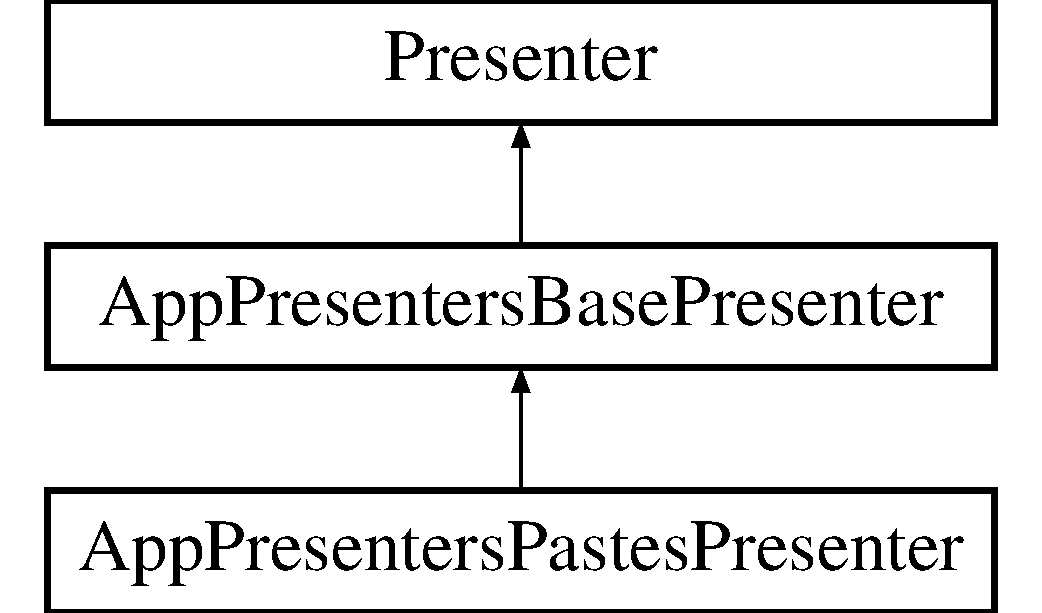
\includegraphics[height=3.000000cm]{classApp_1_1Presenters_1_1PastesPresenter}
\end{center}
\end{figure}
\subsection*{Veřejné metody}
\begin{DoxyCompactItemize}
\item 
\hyperlink{classApp_1_1Presenters_1_1PastesPresenter_a5424badaa457bbf2973cfd41347d906f}{inject\-Models} (\hyperlink{classApp_1_1Model_1_1Pasters}{Model\textbackslash{}\-Pasters} \$\hyperlink{classApp_1_1Model_1_1Pasters}{Pasters})
\begin{DoxyCompactList}\small\item\em Metoda vytvoří pomocí injekce model mapující databázi. \end{DoxyCompactList}\item 
\hypertarget{classApp_1_1Presenters_1_1PastesPresenter_ad79e35733cf83ac8cd097d9f8aab2879}{\hyperlink{classApp_1_1Presenters_1_1PastesPresenter_ad79e35733cf83ac8cd097d9f8aab2879}{render\-Default} ()}\label{classApp_1_1Presenters_1_1PastesPresenter_ad79e35733cf83ac8cd097d9f8aab2879}

\begin{DoxyCompactList}\small\item\em Metoda pro konstrukci proměnných určených pro pohledy. \end{DoxyCompactList}\item 
\hypertarget{classApp_1_1Presenters_1_1PastesPresenter_af4103edcd31b0e1de8ff857dd1e9dda1}{\hyperlink{classApp_1_1Presenters_1_1PastesPresenter_af4103edcd31b0e1de8ff857dd1e9dda1}{action\-Nothing} ()}\label{classApp_1_1Presenters_1_1PastesPresenter_af4103edcd31b0e1de8ff857dd1e9dda1}

\begin{DoxyCompactList}\small\item\em Metoda pro vrácení chyby uživateli přes kontroler flash\-Message. \end{DoxyCompactList}\item 
\hyperlink{classApp_1_1Presenters_1_1PastesPresenter_afa1eed045c70c8e42b187a281aa7d368}{action\-Show} (\$id)
\begin{DoxyCompactList}\small\item\em Metoda z databáze vytáhne všechny pasty podle I\-D. \end{DoxyCompactList}\item 
\hyperlink{classApp_1_1Presenters_1_1PastesPresenter_ad686b8b2060625dabe5f3c19ca22eed8}{action\-Delete} (\$id)
\begin{DoxyCompactList}\small\item\em Metoda z databáze vymaže paste. \end{DoxyCompactList}\end{DoxyCompactItemize}


\subsection{Detailní popis}
Prezentér pro pasty. 

\subsection{Dokumentace k metodám}
\hypertarget{classApp_1_1Presenters_1_1PastesPresenter_ad686b8b2060625dabe5f3c19ca22eed8}{\index{App\-::\-Presenters\-::\-Pastes\-Presenter@{App\-::\-Presenters\-::\-Pastes\-Presenter}!action\-Delete@{action\-Delete}}
\index{action\-Delete@{action\-Delete}!App::Presenters::PastesPresenter@{App\-::\-Presenters\-::\-Pastes\-Presenter}}
\subsubsection[{action\-Delete}]{\setlength{\rightskip}{0pt plus 5cm}App\textbackslash{}\-Presenters\textbackslash{}\-Pastes\-Presenter\-::action\-Delete (
\begin{DoxyParamCaption}
\item[{}]{\$id}
\end{DoxyParamCaption}
)}}\label{classApp_1_1Presenters_1_1PastesPresenter_ad686b8b2060625dabe5f3c19ca22eed8}


Metoda z databáze vymaže paste. 


\begin{DoxyParams}[1]{Parametry}
\mbox{\tt in}  & {\em \$id} & id Pastu \\
\hline
\end{DoxyParams}
\hypertarget{classApp_1_1Presenters_1_1PastesPresenter_afa1eed045c70c8e42b187a281aa7d368}{\index{App\-::\-Presenters\-::\-Pastes\-Presenter@{App\-::\-Presenters\-::\-Pastes\-Presenter}!action\-Show@{action\-Show}}
\index{action\-Show@{action\-Show}!App::Presenters::PastesPresenter@{App\-::\-Presenters\-::\-Pastes\-Presenter}}
\subsubsection[{action\-Show}]{\setlength{\rightskip}{0pt plus 5cm}App\textbackslash{}\-Presenters\textbackslash{}\-Pastes\-Presenter\-::action\-Show (
\begin{DoxyParamCaption}
\item[{}]{\$id}
\end{DoxyParamCaption}
)}}\label{classApp_1_1Presenters_1_1PastesPresenter_afa1eed045c70c8e42b187a281aa7d368}


Metoda z databáze vytáhne všechny pasty podle I\-D. 


\begin{DoxyParams}[1]{Parametry}
\mbox{\tt in}  & {\em \$id} & id Pastu \\
\hline
\end{DoxyParams}
\hypertarget{classApp_1_1Presenters_1_1PastesPresenter_a5424badaa457bbf2973cfd41347d906f}{\index{App\-::\-Presenters\-::\-Pastes\-Presenter@{App\-::\-Presenters\-::\-Pastes\-Presenter}!inject\-Models@{inject\-Models}}
\index{inject\-Models@{inject\-Models}!App::Presenters::PastesPresenter@{App\-::\-Presenters\-::\-Pastes\-Presenter}}
\subsubsection[{inject\-Models}]{\setlength{\rightskip}{0pt plus 5cm}App\textbackslash{}\-Presenters\textbackslash{}\-Pastes\-Presenter\-::inject\-Models (
\begin{DoxyParamCaption}
\item[{{\bf Model\textbackslash{}\-Pasters}}]{\$\-Pasters}
\end{DoxyParamCaption}
)}}\label{classApp_1_1Presenters_1_1PastesPresenter_a5424badaa457bbf2973cfd41347d906f}


Metoda vytvoří pomocí injekce model mapující databázi. 


\begin{DoxyParams}[1]{Parametry}
\mbox{\tt in}  & {\em \$\-Pasters} & injekce modelu \\
\hline
\end{DoxyParams}


Dokumentace pro tuto třídu byla generována z následujícího souboru\-:\begin{DoxyCompactItemize}
\item 
app/presenters/Pastes\-Presenter.\-php\end{DoxyCompactItemize}

\hypertarget{classApp_1_1RouterFactory}{\section{Dokumentace třídy App\textbackslash{}Router\-Factory}
\label{classApp_1_1RouterFactory}\index{App\textbackslash{}\-Router\-Factory@{App\textbackslash{}\-Router\-Factory}}
}
\subsection*{Statické veřejné metody}
\begin{DoxyCompactItemize}
\item 
static \hyperlink{classApp_1_1RouterFactory_a28f3f7de2384fe4101520970c034354d}{create\-Router} ()
\end{DoxyCompactItemize}


\subsection{Dokumentace k metodám}
\hypertarget{classApp_1_1RouterFactory_a28f3f7de2384fe4101520970c034354d}{\index{App\-::\-Router\-Factory@{App\-::\-Router\-Factory}!create\-Router@{create\-Router}}
\index{create\-Router@{create\-Router}!App::RouterFactory@{App\-::\-Router\-Factory}}
\subsubsection[{create\-Router}]{\setlength{\rightskip}{0pt plus 5cm}static App\textbackslash{}\-Router\-Factory\-::create\-Router (
\begin{DoxyParamCaption}
{}
\end{DoxyParamCaption}
)\hspace{0.3cm}{\ttfamily [static]}}}\label{classApp_1_1RouterFactory_a28f3f7de2384fe4101520970c034354d}
\begin{DoxyReturn}{Návratová hodnota}
Nette 
\end{DoxyReturn}


Dokumentace pro tuto třídu byla generována z následujícího souboru\-:\begin{DoxyCompactItemize}
\item 
router/Router\-Factory.\-php\end{DoxyCompactItemize}

\hypertarget{classApp_1_1Forms_1_1SignFormFactory}{\section{Dokumentace třídy App\textbackslash{}Forms\textbackslash{}Sign\-Form\-Factory}
\label{classApp_1_1Forms_1_1SignFormFactory}\index{App\textbackslash{}\-Forms\textbackslash{}\-Sign\-Form\-Factory@{App\textbackslash{}\-Forms\textbackslash{}\-Sign\-Form\-Factory}}
}
Diagram dědičnosti pro třídu App\textbackslash{}Forms\textbackslash{}Sign\-Form\-Factory\begin{figure}[H]
\begin{center}
\leavevmode
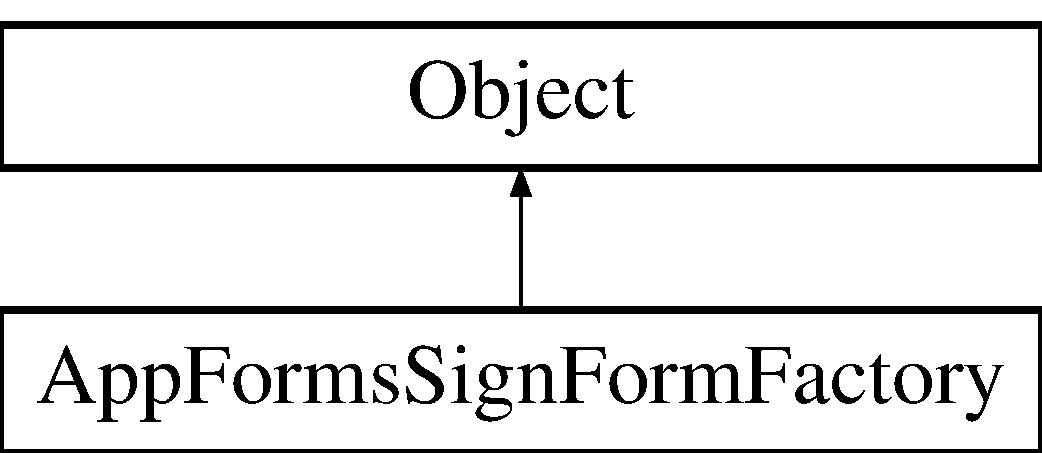
\includegraphics[height=2.000000cm]{classApp_1_1Forms_1_1SignFormFactory}
\end{center}
\end{figure}
\subsection*{Veřejné metody}
\begin{DoxyCompactItemize}
\item 
\hypertarget{classApp_1_1Forms_1_1SignFormFactory_afb6eecdbd9070d6ac6ba5b1d27826832}{{\bfseries \-\_\-\-\_\-construct} (User \$user)}\label{classApp_1_1Forms_1_1SignFormFactory_afb6eecdbd9070d6ac6ba5b1d27826832}

\item 
\hyperlink{classApp_1_1Forms_1_1SignFormFactory_a480cf23c408790dd268e6c06f28723a0}{create} ()
\item 
\hypertarget{classApp_1_1Forms_1_1SignFormFactory_ae3546d8346461c9393200add167d95e2}{{\bfseries form\-Succeeded} (Form \$form, \$values)}\label{classApp_1_1Forms_1_1SignFormFactory_ae3546d8346461c9393200add167d95e2}

\end{DoxyCompactItemize}


\subsection{Dokumentace k metodám}
\hypertarget{classApp_1_1Forms_1_1SignFormFactory_a480cf23c408790dd268e6c06f28723a0}{\index{App\-::\-Forms\-::\-Sign\-Form\-Factory@{App\-::\-Forms\-::\-Sign\-Form\-Factory}!create@{create}}
\index{create@{create}!App::Forms::SignFormFactory@{App\-::\-Forms\-::\-Sign\-Form\-Factory}}
\subsubsection[{create}]{\setlength{\rightskip}{0pt plus 5cm}App\textbackslash{}\-Forms\textbackslash{}\-Sign\-Form\-Factory\-::create (
\begin{DoxyParamCaption}
{}
\end{DoxyParamCaption}
)}}\label{classApp_1_1Forms_1_1SignFormFactory_a480cf23c408790dd268e6c06f28723a0}
\begin{DoxyReturn}{Návratová hodnota}
Form 
\end{DoxyReturn}


Dokumentace pro tuto třídu byla generována z následujícího souboru\-:\begin{DoxyCompactItemize}
\item 
app/forms/Sign\-Form\-Factory.\-php\end{DoxyCompactItemize}

\hypertarget{classApp_1_1Presenters_1_1SignPresenter}{\section{Dokumentace třídy App\textbackslash{}Presenters\textbackslash{}Sign\-Presenter}
\label{classApp_1_1Presenters_1_1SignPresenter}\index{App\textbackslash{}\-Presenters\textbackslash{}\-Sign\-Presenter@{App\textbackslash{}\-Presenters\textbackslash{}\-Sign\-Presenter}}
}
Diagram dědičnosti pro třídu App\textbackslash{}Presenters\textbackslash{}Sign\-Presenter\begin{figure}[H]
\begin{center}
\leavevmode
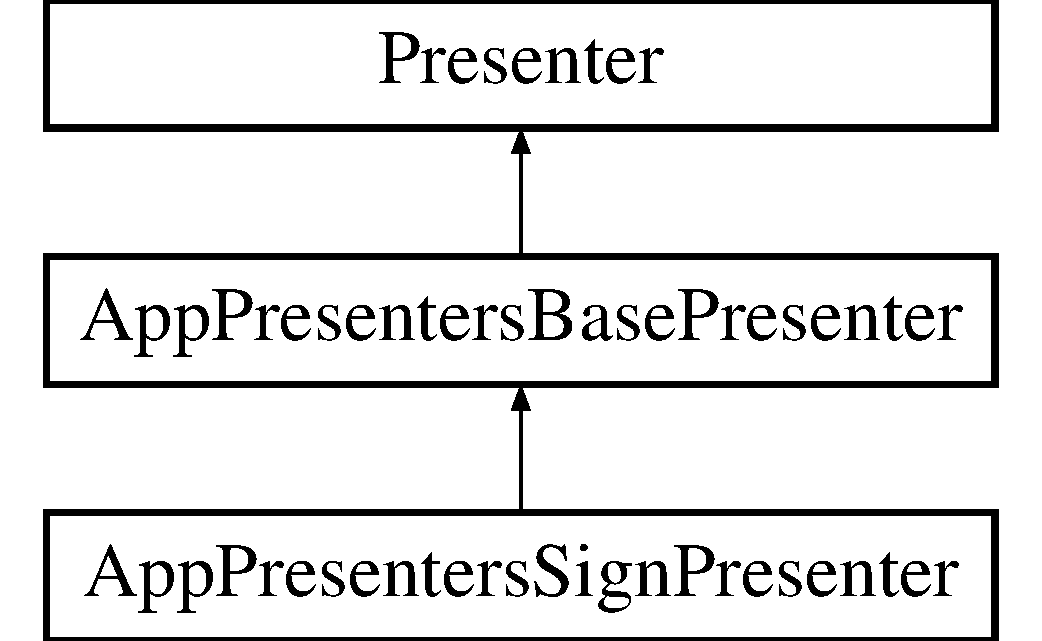
\includegraphics[height=3.000000cm]{classApp_1_1Presenters_1_1SignPresenter}
\end{center}
\end{figure}
\subsection*{Veřejné metody}
\begin{DoxyCompactItemize}
\item 
\hypertarget{classApp_1_1Presenters_1_1SignPresenter_ae9e35c3580aec527734f0839b1fab9fd}{{\bfseries action\-Out} ()}\label{classApp_1_1Presenters_1_1SignPresenter_ae9e35c3580aec527734f0839b1fab9fd}

\end{DoxyCompactItemize}
\subsection*{Veřejné atributy}
\begin{DoxyCompactItemize}
\item 
\hypertarget{classApp_1_1Presenters_1_1SignPresenter_a029117e748148c0452842c23c6fbf0ca}{{\bfseries \$factory}}\label{classApp_1_1Presenters_1_1SignPresenter_a029117e748148c0452842c23c6fbf0ca}

\end{DoxyCompactItemize}
\subsection*{Chráněné metody}
\begin{DoxyCompactItemize}
\item 
\hyperlink{classApp_1_1Presenters_1_1SignPresenter_aa273d99d39b395490fbdfc2702daef38}{create\-Component\-Sign\-In\-Form} ()
\end{DoxyCompactItemize}


\subsection{Dokumentace k metodám}
\hypertarget{classApp_1_1Presenters_1_1SignPresenter_aa273d99d39b395490fbdfc2702daef38}{\index{App\-::\-Presenters\-::\-Sign\-Presenter@{App\-::\-Presenters\-::\-Sign\-Presenter}!create\-Component\-Sign\-In\-Form@{create\-Component\-Sign\-In\-Form}}
\index{create\-Component\-Sign\-In\-Form@{create\-Component\-Sign\-In\-Form}!App::Presenters::SignPresenter@{App\-::\-Presenters\-::\-Sign\-Presenter}}
\subsubsection[{create\-Component\-Sign\-In\-Form}]{\setlength{\rightskip}{0pt plus 5cm}App\textbackslash{}\-Presenters\textbackslash{}\-Sign\-Presenter\-::create\-Component\-Sign\-In\-Form (
\begin{DoxyParamCaption}
{}
\end{DoxyParamCaption}
)\hspace{0.3cm}{\ttfamily [protected]}}}\label{classApp_1_1Presenters_1_1SignPresenter_aa273d99d39b395490fbdfc2702daef38}
Sign-\/in form factory. \begin{DoxyReturn}{Návratová hodnota}
Nette 
\end{DoxyReturn}


Dokumentace pro tuto třídu byla generována z následujícího souboru\-:\begin{DoxyCompactItemize}
\item 
app/presenters/Sign\-Presenter.\-php\end{DoxyCompactItemize}

\hypertarget{classApp_1_1Model_1_1UserManager}{\section{Dokumentace třídy App\textbackslash{}Model\textbackslash{}User\-Manager}
\label{classApp_1_1Model_1_1UserManager}\index{App\textbackslash{}\-Model\textbackslash{}\-User\-Manager@{App\textbackslash{}\-Model\textbackslash{}\-User\-Manager}}
}
Diagram dědičnosti pro třídu App\textbackslash{}Model\textbackslash{}User\-Manager\begin{figure}[H]
\begin{center}
\leavevmode
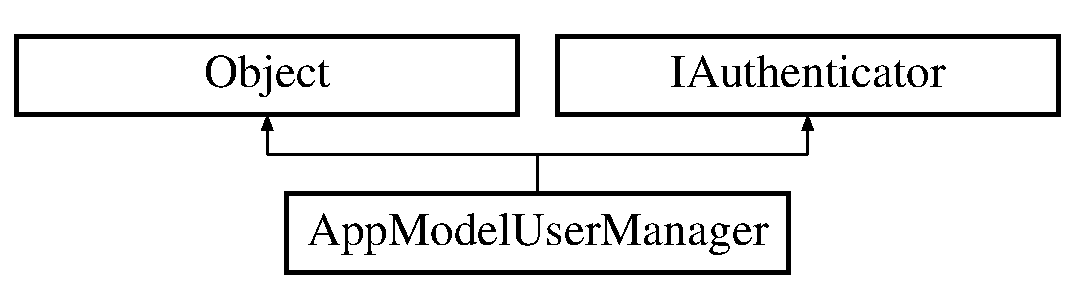
\includegraphics[height=2.000000cm]{classApp_1_1Model_1_1UserManager}
\end{center}
\end{figure}
\subsection*{Veřejné metody}
\begin{DoxyCompactItemize}
\item 
\hypertarget{classApp_1_1Model_1_1UserManager_a23dc73158ccaf8bf52b06acb5178a8d6}{{\bfseries \-\_\-\-\_\-construct} (Nette\textbackslash{}\-Database\textbackslash{}\-Context \$database)}\label{classApp_1_1Model_1_1UserManager_a23dc73158ccaf8bf52b06acb5178a8d6}

\item 
\hyperlink{classApp_1_1Model_1_1UserManager_a77f1c9e747f34dce198c80b6e74cc0ec}{authenticate} (array \$credentials)
\item 
\hyperlink{classApp_1_1Model_1_1UserManager_a83e47d69f7eb85866c86d9e611b9b771}{add} (\$username, \$password)
\item 
\hypertarget{classApp_1_1Model_1_1UserManager_ab9e3b28e92045c329235517f0a75fbef}{{\bfseries rem} (\$username)}\label{classApp_1_1Model_1_1UserManager_ab9e3b28e92045c329235517f0a75fbef}

\end{DoxyCompactItemize}
\subsection*{Veřejné atributy}
\begin{DoxyCompactItemize}
\item 
\hypertarget{classApp_1_1Model_1_1UserManager_ae77830c06b92d32a4948b9e7ef9e5e46}{const {\bfseries T\-A\-B\-L\-E\-\_\-\-N\-A\-M\-E} = 'users'}\label{classApp_1_1Model_1_1UserManager_ae77830c06b92d32a4948b9e7ef9e5e46}

\item 
\hypertarget{classApp_1_1Model_1_1UserManager_a75f9b411c6095d3eb278dc10be81f5e6}{const {\bfseries C\-O\-L\-U\-M\-N\-\_\-\-I\-D} = 'id'}\label{classApp_1_1Model_1_1UserManager_a75f9b411c6095d3eb278dc10be81f5e6}

\item 
\hypertarget{classApp_1_1Model_1_1UserManager_a4019ae437cc39a046444472459631ebd}{const {\bfseries C\-O\-L\-U\-M\-N\-\_\-\-N\-A\-M\-E} = 'username'}\label{classApp_1_1Model_1_1UserManager_a4019ae437cc39a046444472459631ebd}

\item 
\hypertarget{classApp_1_1Model_1_1UserManager_a9c6e473d84c1037c7ec567b6286478fc}{const {\bfseries C\-O\-L\-U\-M\-N\-\_\-\-P\-A\-S\-S\-W\-O\-R\-D\-\_\-\-H\-A\-S\-H} = 'password'}\label{classApp_1_1Model_1_1UserManager_a9c6e473d84c1037c7ec567b6286478fc}

\item 
\hypertarget{classApp_1_1Model_1_1UserManager_af13e6e9c753b0581b42b9305115e5083}{const {\bfseries C\-O\-L\-U\-M\-N\-\_\-\-R\-O\-L\-E} = 'role'}\label{classApp_1_1Model_1_1UserManager_af13e6e9c753b0581b42b9305115e5083}

\end{DoxyCompactItemize}


\subsection{Detailní popis}
Users management. 

\subsection{Dokumentace k metodám}
\hypertarget{classApp_1_1Model_1_1UserManager_a83e47d69f7eb85866c86d9e611b9b771}{\index{App\-::\-Model\-::\-User\-Manager@{App\-::\-Model\-::\-User\-Manager}!add@{add}}
\index{add@{add}!App::Model::UserManager@{App\-::\-Model\-::\-User\-Manager}}
\subsubsection[{add}]{\setlength{\rightskip}{0pt plus 5cm}App\textbackslash{}\-Model\textbackslash{}\-User\-Manager\-::add (
\begin{DoxyParamCaption}
\item[{}]{\$username, }
\item[{}]{\$password}
\end{DoxyParamCaption}
)}}\label{classApp_1_1Model_1_1UserManager_a83e47d69f7eb85866c86d9e611b9b771}
Adds new user. 
\begin{DoxyParams}{Parametry}
{\em string} & \\
\hline
{\em string} & \\
\hline
\end{DoxyParams}
\begin{DoxyReturn}{Návratová hodnota}
void 
\end{DoxyReturn}
\hypertarget{classApp_1_1Model_1_1UserManager_a77f1c9e747f34dce198c80b6e74cc0ec}{\index{App\-::\-Model\-::\-User\-Manager@{App\-::\-Model\-::\-User\-Manager}!authenticate@{authenticate}}
\index{authenticate@{authenticate}!App::Model::UserManager@{App\-::\-Model\-::\-User\-Manager}}
\subsubsection[{authenticate}]{\setlength{\rightskip}{0pt plus 5cm}App\textbackslash{}\-Model\textbackslash{}\-User\-Manager\-::authenticate (
\begin{DoxyParamCaption}
\item[{array}]{\$credentials}
\end{DoxyParamCaption}
)}}\label{classApp_1_1Model_1_1UserManager_a77f1c9e747f34dce198c80b6e74cc0ec}
Performs an authentication. \begin{DoxyReturn}{Návratová hodnota}
Nette 
\end{DoxyReturn}

\begin{DoxyExceptions}{Výjimky}
{\em Nette\textbackslash{}\-Security\textbackslash{}\-Authentication\-Exception} & \\
\hline
\end{DoxyExceptions}


Dokumentace pro tuto třídu byla generována z následujícího souboru\-:\begin{DoxyCompactItemize}
\item 
app/model/User\-Manager.\-php\end{DoxyCompactItemize}

%--- End generated contents ---

% Index
\newpage
\phantomsection
\addcontentsline{toc}{chapter}{Rejstřík}
\printindex

\end{document}
